\documentclass[12pt,a4paper]{article}
\usepackage{amsmath,amssymb,amsfonts}
\usepackage{xcolor}
\usepackage{pgfplots}
\pgfplotsset{compat=newest}
\usetikzlibrary{positioning}

\begin{document}

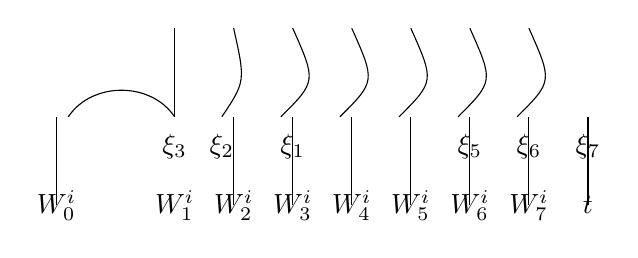
\begin{tikzpicture}[scale=0.75]
    \draw (-1.0,-3.0) node {$W_0^i$};
    \draw (1.0,-3.0) node {$W_1^i$};
    \draw (2.0,-3.0) node {$W_2^i$};
    \draw (3.0,-3.0) node {$W_3^i$};
    \draw (4.0,-3.0) node {$W_4^i$};
    \draw (5.0,-3.0) node {$W_5^i$};
    \draw (6.0,-3.0) node {$W_6^i$};
    \draw (7.0,-3.0) node {$W_7^i$};
    \draw (8.0,-3.0) node {$t$};
    \draw (3.0,-2.0) node {$\xi_1$};
    \draw (1.8,-2.0) node {$\xi_2$};
    \draw (1.0,-2.0) node {$\xi_3$};
    \draw (6.0,-2.0) node {$\xi_5$};
    \draw (7.0,-2.0) node {$\xi_6$};
    \draw (8.0,-2.0) node {$\xi_7$};
    \draw (-1.0,-3.0) -- (-1.0,-1.5);
    \draw (-0.8,-1.5) .. controls (-0.4,-0.9) and (0.6,-0.9) .. (1.0,-1.5);
    \draw (1.0,-1.5) -- (1.0,-0.0);
    \draw (2.0,-3.0) -- (2.0,-1.5);
    \draw (1.8,-1.5) .. controls (2.2,-0.9) and (2.2,-0.9) .. (2.0,-0.0);
    \draw (3.0,-3.0) -- (3.0,-1.5);
    \draw (2.8,-1.5) .. controls (3.4,-0.9) and (3.4,-0.9) .. (3.0,-0.0);
    \draw (4.0,-3.0) -- (4.0,-1.5);
    \draw (3.8,-1.5) .. controls (4.4,-0.9) and (4.4,-0.9) .. (4.0,-0.0);
    \draw (5.0,-3.0) -- (5.0,-1.5);
    \draw (4.8,-1.5) .. controls (5.4,-0.9) and (5.4,-0.9) .. (5.0,-0.0);
    \draw (6.0,-3.0) -- (6.0,-1.5);
    \draw (5.8,-1.5) .. controls (6.4,-0.9) and (6.4,-0.9) .. (6.0,-0.0);
    \draw (7.0,-3.0) -- (7.0,-1.5);
    \draw (6.8,-1.5) .. controls (7.4,-0.9) and (7.4,-0.9) .. (7.0,-0.0);
    \draw (8.0,-3.0) -- (8.0,-1.5);
\end{tikzpicture}

\end{document}